\documentclass[letterpaper,12pt]{article}\usepackage[]{graphicx}\usepackage[]{color}
%% maxwidth is the original width if it is less than linewidth
%% otherwise use linewidth (to make sure the graphics do not exceed the margin)
\makeatletter
\def\maxwidth{ %
  \ifdim\Gin@nat@width>\linewidth
    \linewidth
  \else
    \Gin@nat@width
  \fi
}
\makeatother

\definecolor{fgcolor}{rgb}{0.345, 0.345, 0.345}
\newcommand{\hlnum}[1]{\textcolor[rgb]{0.686,0.059,0.569}{#1}}%
\newcommand{\hlstr}[1]{\textcolor[rgb]{0.192,0.494,0.8}{#1}}%
\newcommand{\hlcom}[1]{\textcolor[rgb]{0.678,0.584,0.686}{\textit{#1}}}%
\newcommand{\hlopt}[1]{\textcolor[rgb]{0,0,0}{#1}}%
\newcommand{\hlstd}[1]{\textcolor[rgb]{0.345,0.345,0.345}{#1}}%
\newcommand{\hlkwa}[1]{\textcolor[rgb]{0.161,0.373,0.58}{\textbf{#1}}}%
\newcommand{\hlkwb}[1]{\textcolor[rgb]{0.69,0.353,0.396}{#1}}%
\newcommand{\hlkwc}[1]{\textcolor[rgb]{0.333,0.667,0.333}{#1}}%
\newcommand{\hlkwd}[1]{\textcolor[rgb]{0.737,0.353,0.396}{\textbf{#1}}}%

\usepackage{framed}
\makeatletter
\newenvironment{kframe}{%
 \def\at@end@of@kframe{}%
 \ifinner\ifhmode%
  \def\at@end@of@kframe{\end{minipage}}%
  \begin{minipage}{\columnwidth}%
 \fi\fi%
 \def\FrameCommand##1{\hskip\@totalleftmargin \hskip-\fboxsep
 \colorbox{shadecolor}{##1}\hskip-\fboxsep
     % There is no \\@totalrightmargin, so:
     \hskip-\linewidth \hskip-\@totalleftmargin \hskip\columnwidth}%
 \MakeFramed {\advance\hsize-\width
   \@totalleftmargin\z@ \linewidth\hsize
   \@setminipage}}%
 {\par\unskip\endMakeFramed%
 \at@end@of@kframe}
\makeatother

\definecolor{shadecolor}{rgb}{.97, .97, .97}
\definecolor{messagecolor}{rgb}{0, 0, 0}
\definecolor{warningcolor}{rgb}{1, 0, 1}
\definecolor{errorcolor}{rgb}{1, 0, 0}
\newenvironment{knitrout}{}{} % an empty environment to be redefined in TeX

\usepackage{alltt}
\usepackage[top=1in,bottom=1in,left=1in,right=1in]{geometry}
\usepackage{setspace}
\usepackage[colorlinks=true,urlcolor=blue,citecolor=blue,linkcolor=blue]{hyperref}
\usepackage{indentfirst}
\usepackage{multirow}
\usepackage{booktabs}
\usepackage[final]{animate}
\usepackage{graphicx}
\usepackage{verbatim}
\usepackage{rotating}
\usepackage{tabularx}
\usepackage{array}
\usepackage{subfig} 
\usepackage[noae]{Sweave}
\usepackage{cleveref}
\usepackage[figureposition=bottom]{caption}
\usepackage{paralist}
\usepackage{acronym}
\usepackage{outlines}
\usepackage{pdflscape}

%for supplemental figures/tables
\newcommand{\beginsupplement}{%
        \setcounter{table}{0}
        \renewcommand{\thetable}{S\arabic{table}}%
        \setcounter{figure}{0}
        \renewcommand{\thefigure}{S\arabic{figure}}%
     }

% knitr options




\IfFileExists{upquote.sty}{\usepackage{upquote}}{}
\begin{document}

\setcounter{figure}{1}
\setcounter{table}{1}

\begin{landscape}
\centering\vspace*{\fill}
\begin{figure}[!ht]

{\centering 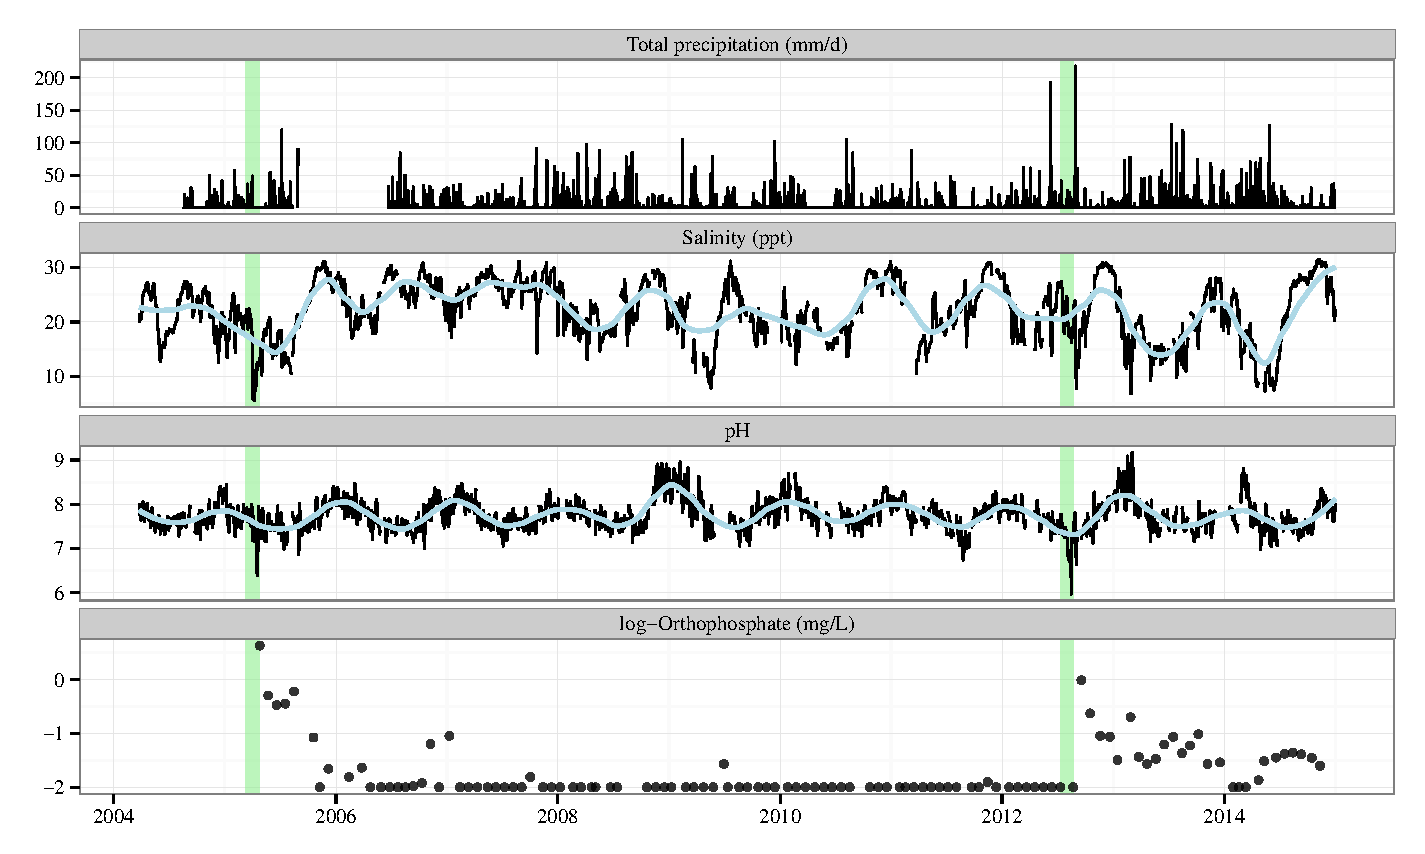
\includegraphics[width=\maxwidth,height=4.8in]{figs/tsplot-1} 

}

\caption[Time series of total precipitation, salinity, pH, and phosphate for Bangs Lake, Grand Bay reserve]{Time series of total precipitation, salinity, pH, and phosphate for Bangs Lake, Grand Bay reserve.  All observations are daily averages, excluding phosphate which was sampled monthly.  Vertical green bars indicate a heavy rain event in April 2005 and hurricane Isaac in August 2012.  Salinity and pH include a loess smooth to reduce variability. Orthophosphate is colored by event categories in relation to the vertical green bars.  E1A: event 1 acute, E1C: event 1 chronic, NI: non-impact, E2A: event 2 acute, E2C: event 2 chronic.}\label{fig:tsplot}
\end{figure}


\end{landscape}
\clearpage

\begin{figure}[!ht]

{\centering 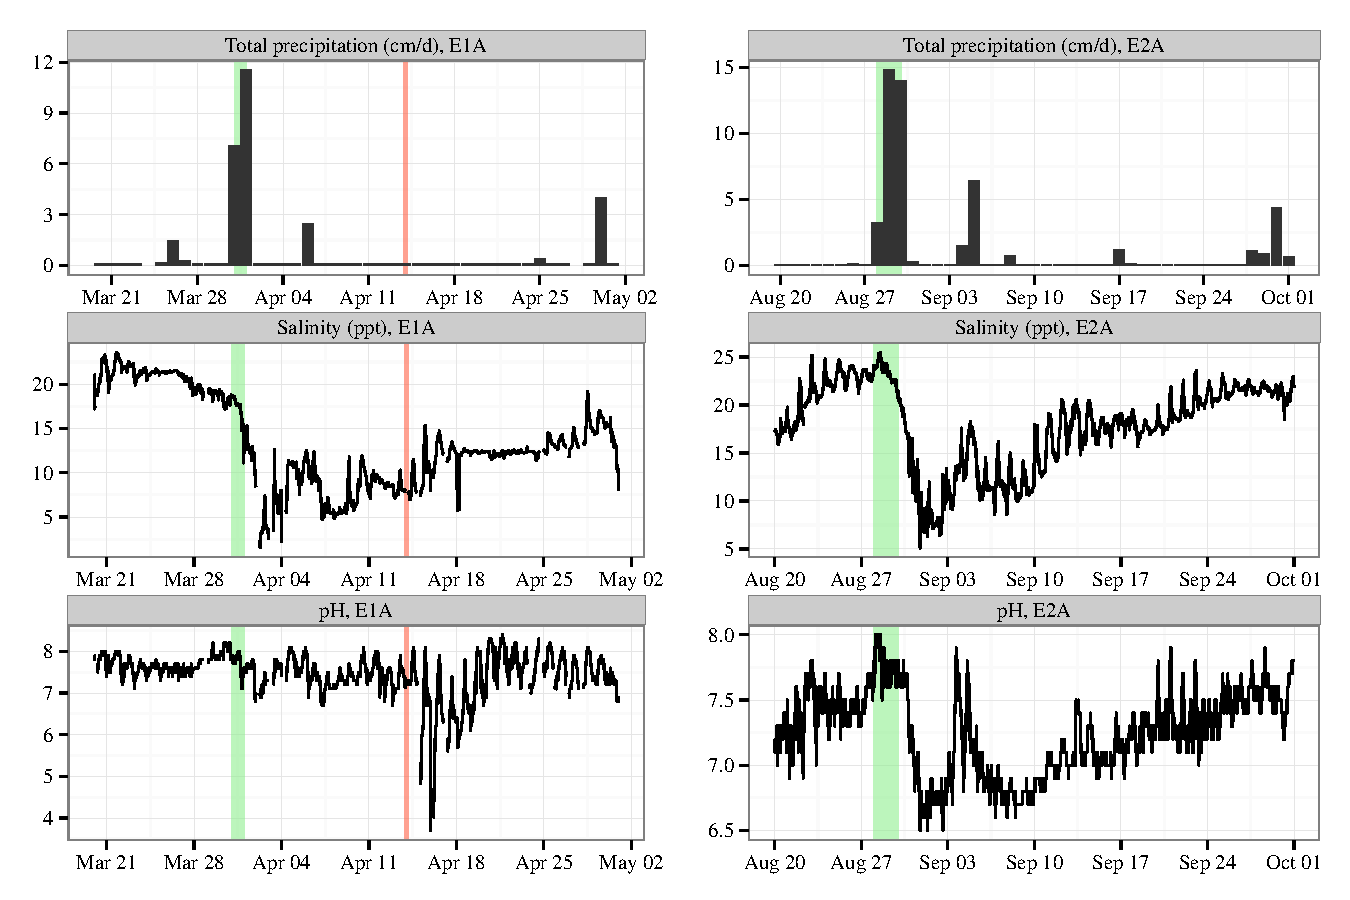
\includegraphics[width=\maxwidth]{figs/tsplotexp-1} 

}

\caption[Time series of daily precipitation, salinity, and pH for Bangs Lake, Grand Bay reserve]{Time series of daily precipitation, salinity, and pH for Bangs Lake, Grand Bay reserve.  Precipitation data represents daily totals from the Pascagoula International Airport.  Salinity and pH data were collected at 15 minute time steps.  Green shading indicates period of high precipitation for a heavy rain event in 2005 (left, March 31\textsuperscript{st} to April 1\textsuperscript{st}) and hurricane Isaac in 2012 (right, August 28\textsuperscript{th} to 30\textsuperscript{th}).  Red shading for the first event indicates the date of documented phosphorus spill.  E1A: event 1 acute, E2A: event 2 acute.}\label{fig:tsplotexp}
\end{figure}


\clearpage

\begin{figure}[!ht]

{\centering 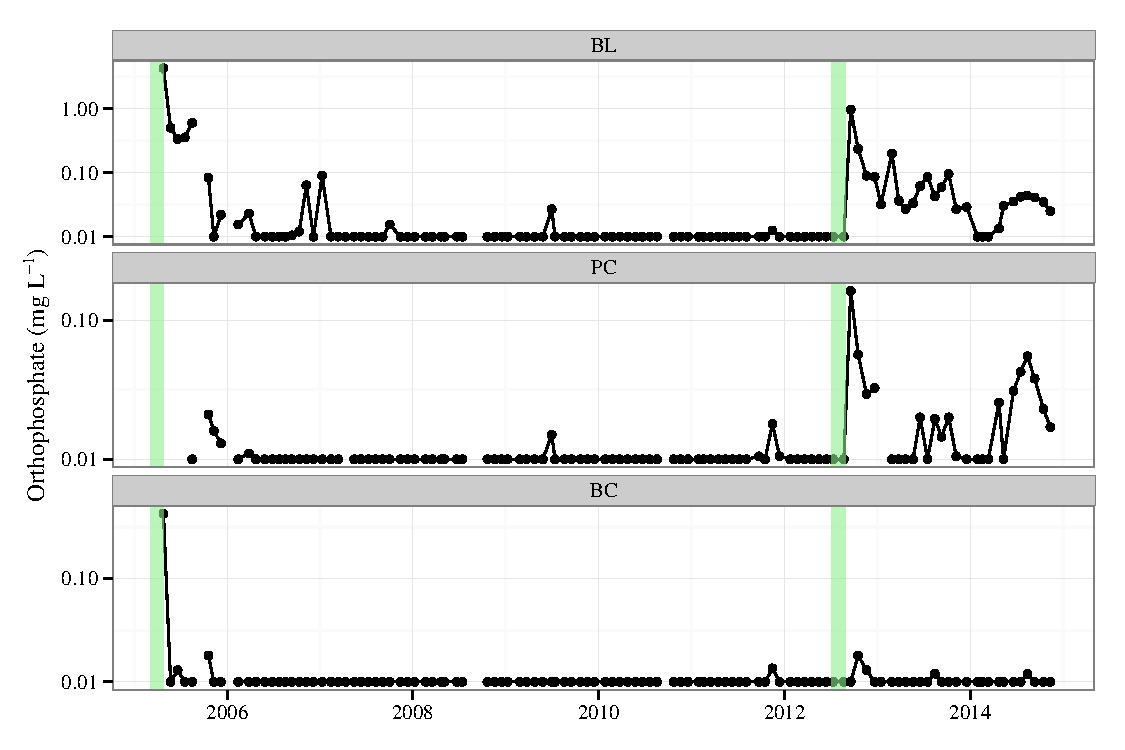
\includegraphics[width=\maxwidth]{figs/orthtsfig-1} 

}

\caption[Monthly phosphate time series at Bangs Lake (BL), Point aux Chenes (PC), and Bayou Cumbest (BC) sites at Grand Bay]{Monthly phosphate time series at Bangs Lake (BL), Point aux Chenes (PC), and Bayou Cumbest (BC) sites at Grand Bay. Vertical green bars indicate a heavy rain event in April 2005 and hurricane Isaac in August 2012.}\label{fig:orthtsfig}
\end{figure}


\clearpage

\begin{figure}[!ht]

{\centering 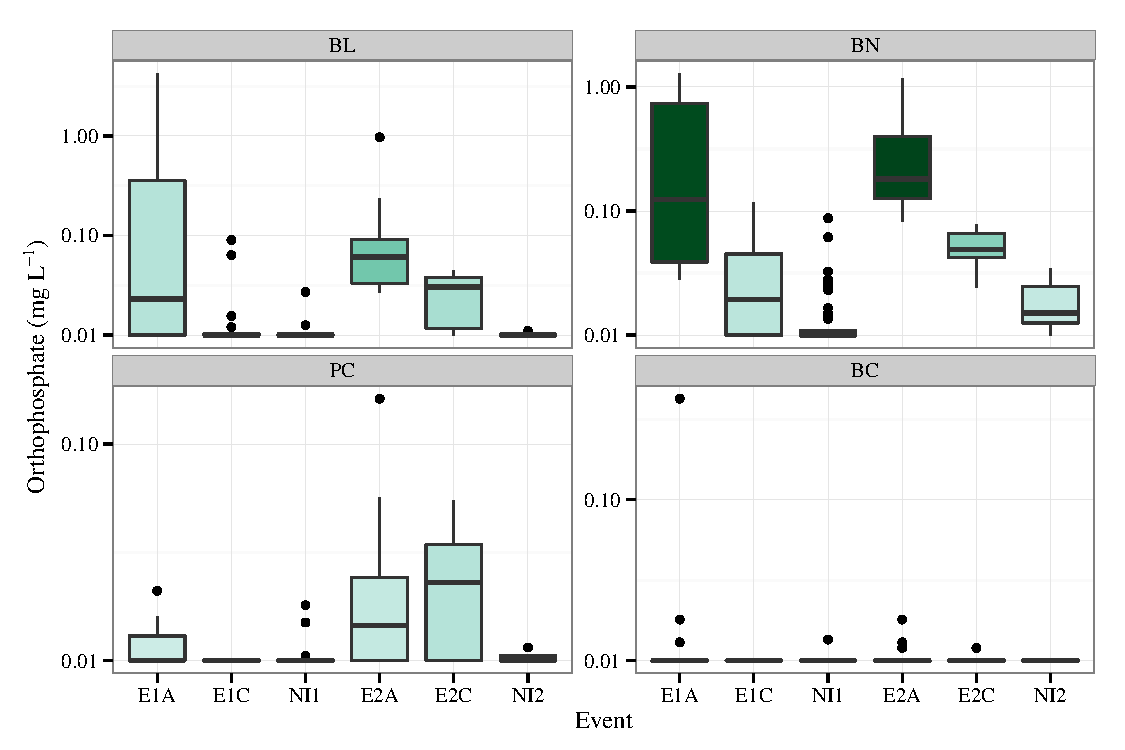
\includegraphics[width=\maxwidth]{figs/orthfig-1} 

}

\caption{Boxplot summaries by event of monthly orthophosphate data at Bangs Lake (BL), and Point aux Chenes (PC), and Bayou Cumbest (BC) sites in Grand Bay.  Boxes represent the interquartile range (IQR, 25\textsuperscript{th} to 75\textsuperscript{th} percentile) with the median as the middle horizonal line.  Outliers are present beyond whiskers (1.5$\cdot$IQR). Boxes are shaded by medians between sites.  See \cref{tab:orthtab} for a numerical summary. E1A: event 1 acute, E1C: event 1 chronic, NI: non-impact, E2A: event 2 acute, E2C: event 2 chronic.}\label{fig:orthfig}
\end{figure}


\clearpage

\begin{figure}[!ht]

{\centering 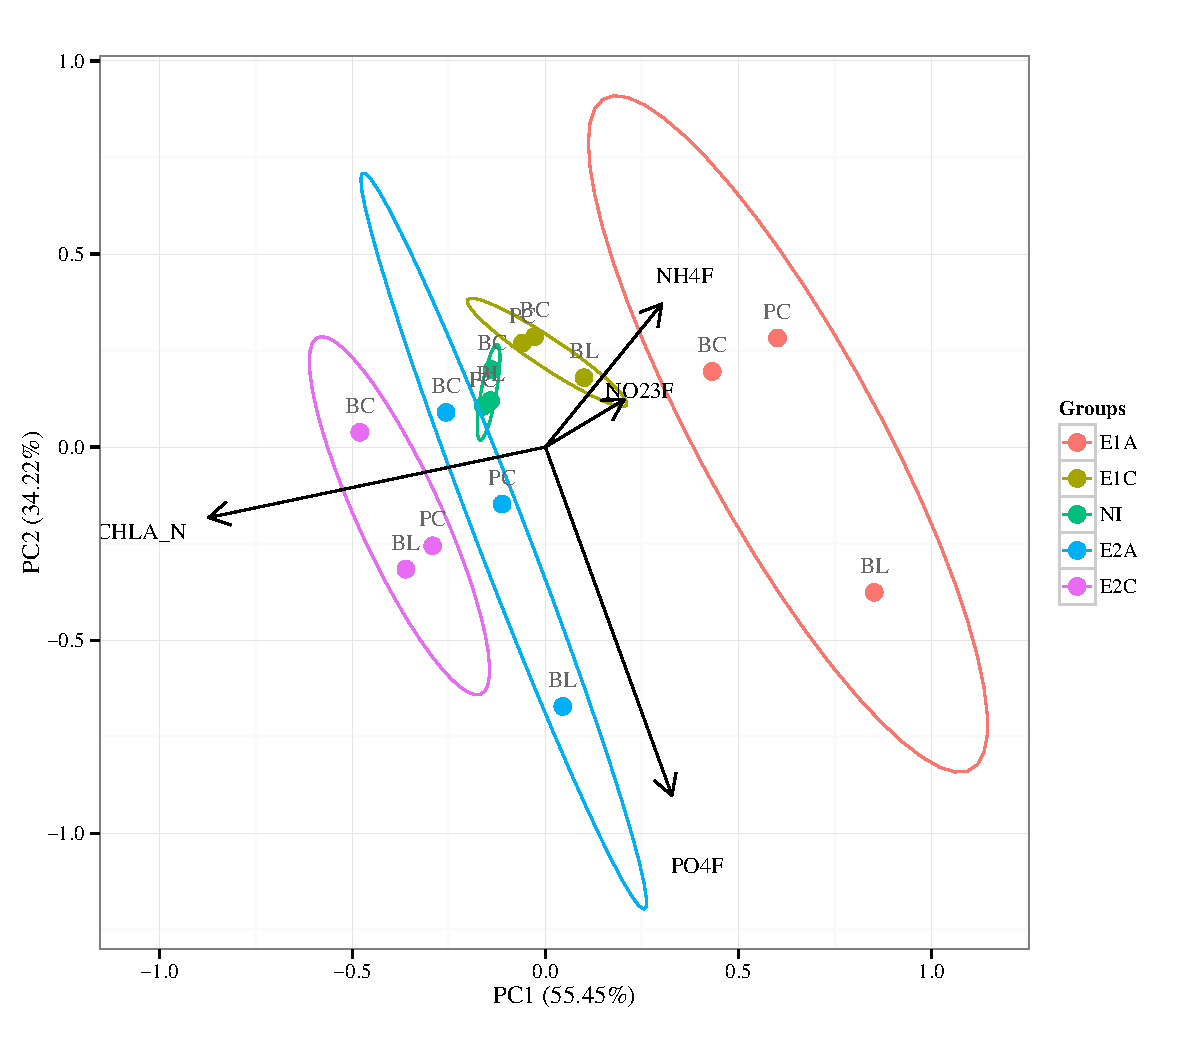
\includegraphics[width=\maxwidth]{figs/pcafig-1} 

}

\caption[Ordination biplot of nutrient values by site and time frames]{Ordination biplot of nutrient values by site and time frames. Monthly data were averaged by site and time frame prior to ordination.  Site are Bangs Lake (BL), Point aux Chenes (PC), and Bayou Cumbest (BC). E1A: event 1 acute, E1C: event 1 chronic, NI: non-impact, E2A: event 2 acute, E2C: event 2 chronic.}\label{fig:pcafig}
\end{figure}


\clearpage

%latex.default(tab, file = "", rowlabel = "Site", caption = cap,     caption.loc = "top", rgroup = unique(res$StationCode), n.rgroup = rep(5,         3), rowname = rows, colheads = c("Result", "Mean", "St. Dev.",         "n", "Min", "Max"), label = "tab:orthtab")%
\begin{table}[!tbp]
\caption{Summaries by site and event of monthly orthophosphate data at Bayou Cumbest (BC), Bangs Lake (BL), and Point aux Chenes (PC) in Grand Bay.  Values are within-group summaries of mean, standard deviation, sample size, and range for orthophosphate by station and time frame.  Result letters indicate time frames within each station that were not significantly different based on Tukey multiple comparison analyses ($\alpha = 0.05$, corrected to reduce Type I error rates). Timeframes are E1A: event 1 acute, E1C: event 1 chronic, NI: non-impact, E2A: event 2 acute, E2C: event 2 chronic.\label{tab:orthtab}} 
\begin{center}
\begin{tabular}{llrrrrr}
\hline\hline
\multicolumn{1}{l}{Site}&\multicolumn{1}{c}{Result}&\multicolumn{1}{c}{Mean}&\multicolumn{1}{c}{St. Dev.}&\multicolumn{1}{c}{n}&\multicolumn{1}{c}{Min}&\multicolumn{1}{c}{Max}\tabularnewline
\hline
{\bfseries BL}&&&&&&\tabularnewline
~~E1A&a&$0.07$&$7.80$&$13$&$0.01$&$4.29$\tabularnewline
~~E1C&bc&$0.01$&$1.89$&$19$&$0.01$&$0.09$\tabularnewline
~~NI&c&$0.01$&$1.15$&$52$&$0.01$&$0.03$\tabularnewline
~~E2A&a&$0.07$&$2.64$&$16$&$0.03$&$0.97$\tabularnewline
~~E2C&b&$0.02$&$1.87$&$11$&$0.01$&$0.04$\tabularnewline
\hline
{\bfseries PC}&&&&&&\tabularnewline
~~E1A&bc&$0.01$&$1.31$&$ 9$&$0.01$&$0.02$\tabularnewline
~~E1C&c&$0.01$&$1.00$&$18$&$0.01$&$0.01$\tabularnewline
~~NI&c&$0.01$&$1.10$&$52$&$0.01$&$0.02$\tabularnewline
~~E2A&ab&$0.02$&$2.24$&$15$&$0.01$&$0.16$\tabularnewline
~~E2C&a&$0.02$&$1.91$&$11$&$0.01$&$0.06$\tabularnewline
\hline
{\bfseries BC}&&&&&&\tabularnewline
~~E1A&a&$0.01$&$2.82$&$13$&$0.01$&$0.43$\tabularnewline
~~E1C&b&$0.01$&$1.00$&$19$&$0.01$&$0.01$\tabularnewline
~~NI&b&$0.01$&$1.04$&$52$&$0.01$&$0.01$\tabularnewline
~~E2A&ab&$0.01$&$1.17$&$16$&$0.01$&$0.02$\tabularnewline
~~E2C&ab&$0.01$&$1.06$&$11$&$0.01$&$0.01$\tabularnewline
\hline
\end{tabular}\end{center}

\end{table}

\clearpage

% supplements
\beginsupplement

\begin{figure}[!ht]

{\centering 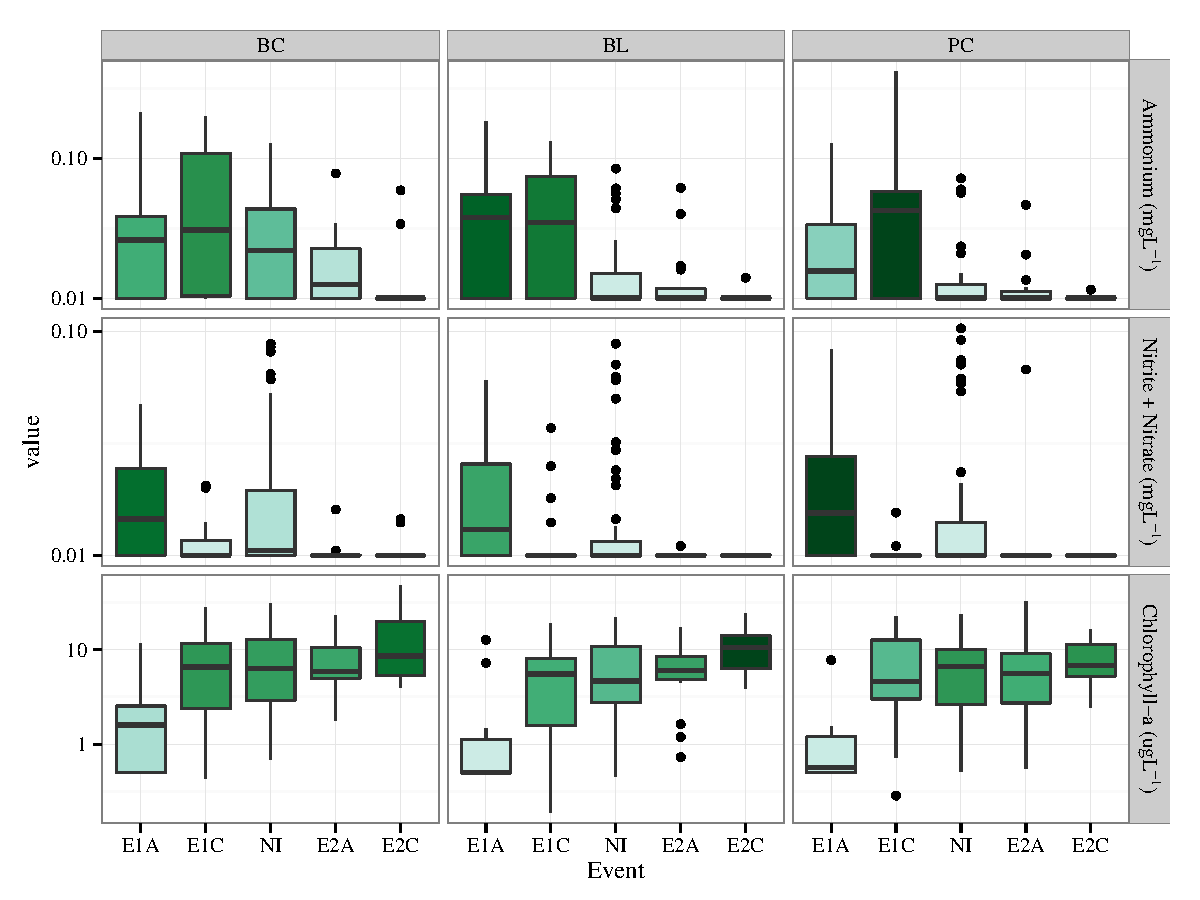
\includegraphics[width=\maxwidth]{figs/boxplt_all-1} 

}

\caption{Boxplot summaries by event of nutrient data at Bayou Cumbest (BC), Bangs Lake (BL), and Point aux Chenes (PC) sites at Grand Bay.  Boxes represent the interquartile range (IQR, 25\textsuperscript{th} to 75\textsuperscript{th} percentile) with the median as the middle horizonal line.  Boxes are colored by relative median nutrients between sites.  Outliers are present beyond whiskers (1.5$\cdot$IQR). See \cref{tab:ammontab,tab:tntab,tab:chltab} for numerical summaries.  E1A: event 1 acute, E1C: event 1 chronic, NI: non-impact, E2A: event 2 acute, E2C: event 2 chronic.}\label{fig:boxplt_all}
\end{figure}


\clearpage

%latex.default(tab, file = "", rowlabel = "Site", caption = cap,     caption.loc = "top", rgroup = unique(res$StationCode), n.rgroup = rep(5,         3), rowname = rows, colheads = c("Result", "Mean", "St. Dev.",         "n", "Min", "Max"), label = "tab:ammontab")%
\begin{table}[!tbp]
\caption{Summaries by site and event of monthly ammonium data at Bayou Cumbest (BC), Bangs Lake (BL), and Point aux Chenes (PC) in Grand Bay.  Values are within-group summaries of mean, standard deviation, sample size, and range for ammonium by station and time frame.  Result letters indicate time frames within each station that were not significantly different based on Tukey multiple comparison analyses ($\alpha = 0.05$, corrected to reduce Type I error rates). Timeframes are E1A: event 1 acute, E1C: event 1 chronic, NI: non-impact, E2A: event 2 acute, E2C: event 2 chronic.\label{tab:ammontab}} 
\begin{center}
\begin{tabular}{llrrrrr}
\hline\hline
\multicolumn{1}{l}{Site}&\multicolumn{1}{c}{Result}&\multicolumn{1}{c}{Mean}&\multicolumn{1}{c}{St. Dev.}&\multicolumn{1}{c}{n}&\multicolumn{1}{c}{Min}&\multicolumn{1}{c}{Max}\tabularnewline
\hline
{\bfseries BL}&&&&&&\tabularnewline
~~E1A&a&$0.03$&$2.72$&$12$&$0.01$&$0.18$\tabularnewline
~~E1C&a&$0.03$&$2.64$&$18$&$0.01$&$0.13$\tabularnewline
~~NI&b&$0.01$&$1.74$&$49$&$0.01$&$0.08$\tabularnewline
~~E2A&b&$0.01$&$1.74$&$16$&$0.01$&$0.06$\tabularnewline
~~E2C&b&$0.01$&$1.11$&$11$&$0.01$&$0.01$\tabularnewline
\hline
{\bfseries PC}&&&&&&\tabularnewline
~~E1A&ab&$0.02$&$2.52$&$ 8$&$0.01$&$0.13$\tabularnewline
~~E1C&a&$0.04$&$3.06$&$17$&$0.01$&$0.42$\tabularnewline
~~NI&b&$0.01$&$1.59$&$49$&$0.01$&$0.07$\tabularnewline
~~E2A&b&$0.01$&$1.50$&$16$&$0.01$&$0.05$\tabularnewline
~~E2C&b&$0.01$&$1.04$&$11$&$0.01$&$0.01$\tabularnewline
\hline
{\bfseries BC}&&&&&&\tabularnewline
~~E1A&ab&$0.03$&$2.63$&$12$&$0.01$&$0.21$\tabularnewline
~~E1C&a&$0.04$&$3.13$&$18$&$0.01$&$0.20$\tabularnewline
~~NI&ab&$0.02$&$2.15$&$49$&$0.01$&$0.13$\tabularnewline
~~E2A&b&$0.02$&$1.79$&$16$&$0.01$&$0.08$\tabularnewline
~~E2C&b&$0.01$&$1.86$&$11$&$0.01$&$0.06$\tabularnewline
\hline
\end{tabular}\end{center}

\end{table}

\clearpage

%latex.default(tab, file = "", rowlabel = "Site", caption = cap,     caption.loc = "top", rgroup = unique(res$StationCode), n.rgroup = rep(5,         3), rowname = rows, colheads = c("Result", "Mean", "St. Dev.",         "n", "Min", "Max"), label = "tab:tntab")%
\begin{table}[!tbp]
\caption{Summaries by site and event of monthly total nitrogen (nitrate, nitrite) data at Bayou Cumbest (BC), Bangs Lake (BL), and Point aux Chenes (PC) in Grand Bay.  Values are within-group summaries of mean, standard deviation, sample size, and range for total nitrogen by station and time frame.  Result letters indicate time frames within each station that were not significantly different based on Tukey multiple comparison analyses ($\alpha = 0.05$, corrected to reduce Type I error rates). Timeframes are E1A: event 1 acute, E1C: event 1 chronic, NI: non-impact, E2A: event 2 acute, E2C: event 2 chronic.\label{tab:tntab}} 
\begin{center}
\begin{tabular}{llrrrrr}
\hline\hline
\multicolumn{1}{l}{Site}&\multicolumn{1}{c}{Result}&\multicolumn{1}{c}{Mean}&\multicolumn{1}{c}{St. Dev.}&\multicolumn{1}{c}{n}&\multicolumn{1}{c}{Min}&\multicolumn{1}{c}{Max}\tabularnewline
\hline
{\bfseries BL}&&&&&&\tabularnewline
~~E1A&a&$0.02$&$1.86$&$14$&$0.01$&$0.06$\tabularnewline
~~E1C&ab&$0.01$&$1.45$&$19$&$0.01$&$0.04$\tabularnewline
~~NI&ab&$0.01$&$1.80$&$53$&$0.01$&$0.09$\tabularnewline
~~E2A&b&$0.01$&$1.02$&$15$&$0.01$&$0.01$\tabularnewline
~~E2C&b&$0.01$&$1.00$&$11$&$0.01$&$0.01$\tabularnewline
\hline
{\bfseries PC}&&&&&&\tabularnewline
~~E1A&a&$0.02$&$2.31$&$10$&$0.01$&$0.08$\tabularnewline
~~E1C&b&$0.01$&$1.11$&$18$&$0.01$&$0.02$\tabularnewline
~~NI&ab&$0.01$&$1.95$&$53$&$0.01$&$0.10$\tabularnewline
~~E2A&ab&$0.01$&$1.64$&$15$&$0.01$&$0.07$\tabularnewline
~~E2C&b&$0.01$&$1.00$&$11$&$0.01$&$0.01$\tabularnewline
\hline
{\bfseries BC}&&&&&&\tabularnewline
~~E1A&a&$0.02$&$1.79$&$14$&$0.01$&$0.05$\tabularnewline
~~E1C&ab&$0.01$&$1.26$&$19$&$0.01$&$0.02$\tabularnewline
~~NI&a&$0.02$&$1.94$&$53$&$0.01$&$0.09$\tabularnewline
~~E2A&ab&$0.01$&$1.12$&$16$&$0.01$&$0.02$\tabularnewline
~~E2C&ab&$0.01$&$1.15$&$11$&$0.01$&$0.01$\tabularnewline
\hline
\end{tabular}\end{center}

\end{table}

\clearpage

%latex.default(tab, file = "", rowlabel = "Site", caption = cap,     caption.loc = "top", rgroup = unique(res$StationCode), n.rgroup = rep(5,         3), rowname = rows, colheads = c("Result", "Mean", "St. Dev.",         "n", "Min", "Max"), label = "tab:chltab")%
\begin{table}[!tbp]
\caption{Summaries by site and event of monthly chlorophyll data at Bayou Cumbest (BC), Bangs Lake (BL), and Point aux Chenes (PC) in Grand Bay.  Values are within-group summaries of mean, standard deviation, sample size, and range for chlorophyll by station and time frame.  Result letters indicate time frames within each station that were not significantly different based on Tukey multiple comparison analyses ($\alpha = 0.05$, corrected to reduce Type I error rates). Timeframes are E1A: event 1 acute, E1C: event 1 chronic, NI: non-impact, E2A: event 2 acute, E2C: event 2 chronic.\label{tab:chltab}} 
\begin{center}
\begin{tabular}{llrrrrr}
\hline\hline
\multicolumn{1}{l}{Site}&\multicolumn{1}{c}{Result}&\multicolumn{1}{c}{Mean}&\multicolumn{1}{c}{St. Dev.}&\multicolumn{1}{c}{n}&\multicolumn{1}{c}{Min}&\multicolumn{1}{c}{Max}\tabularnewline
\hline
{\bfseries BL}&&&&&&\tabularnewline
~~E1A&b&$ 0.94$&$2.87$&$14$&$0.50$&$12.68$\tabularnewline
~~E1C&a&$ 3.39$&$3.61$&$18$&$0.19$&$18.89$\tabularnewline
~~NI&a&$ 4.60$&$2.58$&$54$&$0.46$&$21.99$\tabularnewline
~~E2A&a&$ 5.35$&$2.39$&$16$&$0.73$&$17.28$\tabularnewline
~~E2C&a&$ 9.44$&$1.84$&$11$&$3.90$&$23.89$\tabularnewline
\hline
{\bfseries PC}&&&&&&\tabularnewline
~~E1A&b&$ 0.87$&$2.41$&$10$&$0.50$&$ 7.74$\tabularnewline
~~E1C&a&$ 4.85$&$3.26$&$17$&$0.29$&$22.56$\tabularnewline
~~NI&a&$ 4.73$&$2.66$&$54$&$0.52$&$23.39$\tabularnewline
~~E2A&a&$ 4.88$&$2.66$&$16$&$0.55$&$32.52$\tabularnewline
~~E2C&a&$ 7.48$&$1.79$&$11$&$2.44$&$16.46$\tabularnewline
\hline
{\bfseries BC}&&&&&&\tabularnewline
~~E1A&b&$ 1.52$&$3.02$&$13$&$0.50$&$11.75$\tabularnewline
~~E1C&a&$ 4.64$&$3.55$&$18$&$0.44$&$28.02$\tabularnewline
~~NI&a&$ 5.58$&$2.78$&$54$&$0.69$&$30.59$\tabularnewline
~~E2A&a&$ 6.29$&$2.15$&$16$&$1.78$&$23.12$\tabularnewline
~~E2C&a&$10.49$&$2.34$&$11$&$3.93$&$47.67$\tabularnewline
\hline
\end{tabular}\end{center}

\end{table}

\clearpage

\end{document}
